\part{Wintersemester 2009}
\chapter{Physik (PH)}
\section{2009.10.05}
\section{IMG1}
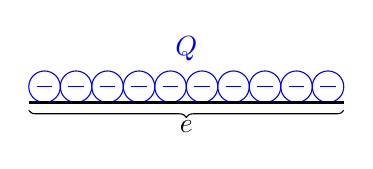
\begin{tikzpicture}
\foreach \x in {0.2,0.6,...,4}
{
	\draw[color=blue] (\x,0.2) circle (0.2);
	\draw[color=blue] (\x-0.1,0.2) -- (\x+0.1,0.2);
}
\draw[thick] (0,0) -- (4,0);
\node[color=blue] at (2,0.4) [above] {$Q$};
\draw decorate [decoration=brace] {(4,-0.1) -- (0,-0.1) node[below,midway] {$e$}};
\end{tikzpicture}

\section{IMG2}
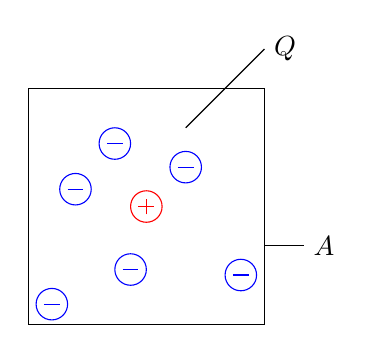
\begin{tikzpicture}
%Negative Ladungen
\foreach \x/\y in
{
0.3/0.26,
0.6/1.72,
2.7/0.63,
2/2,
1.3/0.7,
1.1/2.3
}
{
	\draw[color=blue] (\x,\y) circle (0.2);
	\draw[color=blue] (\x-0.1,\y) -- (\x+0.1,\y);
}

%Positive Ladungen
\foreach \x/\y in
{
1.5/1.5
}
{
	\draw[color=red] (\x,\y) circle (0.2);
	\draw[color=red] (\x-0.1,\y) -- (\x+0.1,\y);
	\draw[color=red] (\x,\y-0.1) -- (\x,\y+0.1);
}

\draw (0,0) rectangle (3,3);

\draw(2,2.5) -- (3,3.5) node[right] {$Q$};
\draw(3,1) -- (3.5,1) node[right] {$A$};

\end{tikzpicture}

\section{IMG3}
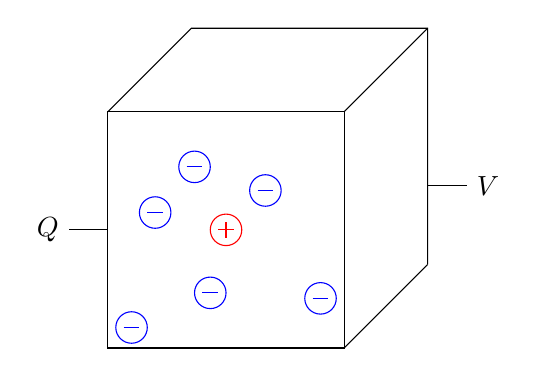
\begin{tikzpicture}
%Negative Ladungen
\foreach \x/\y in
{
0.3/0.26,
0.6/1.72,
2.7/0.63,
2/2,
1.3/0.7,
1.1/2.3
}
{
	\draw[color=blue] (\x,\y) circle (0.2);
	\draw[color=blue] (\x-0.1,\y) -- (\x+0.1,\y);
}

%Positive Ladungen
\foreach \x/\y in
{
1.5/1.5
}
{
	\draw[color=red] (\x,\y) circle (0.2);
	\draw[color=red] (\x-0.1,\y) -- (\x+0.1,\y);
	\draw[color=red] (\x,\y-0.1) -- (\x,\y+0.1);
}

\draw (0,0) rectangle (3,3);
\draw (3,3) -- ++(45:1.5);
\draw (3,0) -- ++(45:1.5);
\draw (0,3) -- ++(45:1.5) -- ++(3,0) -- ++(0,-3);

\draw(0,1.5) -- (-0.5,1.5) node[left] {$Q$};
\draw(3,1) ++(45:1.5) -- ++(0.5,0) node[right] {$V$};

\end{tikzpicture}


\chapter{Mathematik 1 (MA1)}
